%%% LaTeX Template: Article/Thesis/etc. with colored headings and special fonts
%%%
%%% Source: http://www.howtotex.com/
%%% Feel free to distribute this template, but please keep to referal to http://www.howtotex.com/ here.
%%% February 2011
%%%
%%% Modified May 2018 by CDM

%%%  Preamble
\documentclass[11pt,letterpaper]{article}
\usepackage[margin=1.0in]{geometry}
\usepackage[T1]{fontenc}
\usepackage[bitstream-charter]{mathdesign}
\usepackage[latin1]{inputenc}					
\usepackage{amsmath}						
\usepackage{xcolor}
\usepackage{cite}
\usepackage{hyphenat}
\usepackage{graphicx}
\usepackage{float}
\usepackage{subfigure}
\usepackage{sectsty}
\usepackage[compact]{titlesec} 
\usepackage[tablegrid]{vhistory}
\allsectionsfont{\color{accentcolor}\scshape\selectfont}

%%% Definitions
\definecolor{accentcolor}{rgb}{0.0,0.0,0.5} 
\newcommand{\teamname}{Team Name}
\newcommand{\productname}{Product Name}
\newcommand{\coursename}{CSE 4316: Senior Design I}
\newcommand{\semester}{Spring 2018}
\newcommand{\docname}{System Requirements Specification}
\newcommand{\department}{Department of Computer Science \& Engineering}
\newcommand{\university}{The University of Texas at Arlington}
\newcommand{\authors}{Alan Turing \\ Grace Hopper \\ John Von Neumann \\ Ada Lovelace \\ Charles Babbage}

%%% Headers and footers
\usepackage{fancyhdr}
	\pagestyle{fancy}						% Enabling the custom headers/footers
\usepackage{lastpage}	
	% Header (empty)
	\lhead{}
	\chead{}
	\rhead{}
	% Footer
	\lfoot{\footnotesize \teamname \ - \semester}
	\cfoot{}
	\rfoot{\footnotesize page \thepage\ of \pageref{LastPage}}	% "Page 1 of 2"
	\renewcommand{\headrulewidth}{0.0pt}
	\renewcommand{\footrulewidth}{0.4pt}

%%% Change the abstract environment
\usepackage[runin]{abstract}			% runin option for a run-in title
%\setlength\absleftindent{30pt}			% left margin
%\setlength\absrightindent{30pt}		% right margin
\abslabeldelim{\quad}	
\setlength{\abstitleskip}{-10pt}
\renewcommand{\abstractname}{}
\renewcommand{\abstracttextfont}{\color{accentcolor} \small \slshape}	% slanted text

%%% Start of the document
\begin{document}

%%% Cover sheet
{\centering \huge \color{accentcolor} \sc \textbf{\department \\ \university} \par}
\vspace{1 in}
{\centering \huge \color{accentcolor} \sc \textbf{\docname \\ \coursename \\ \semester} \par}
\vspace{0.5 in}
\begin{figure}[h!]
	\centering
   	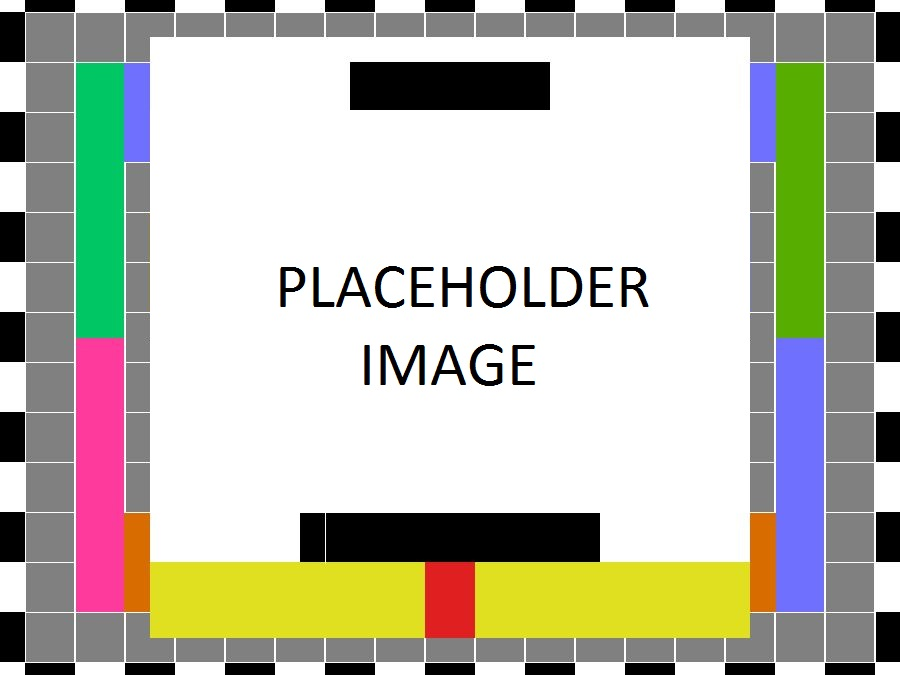
\includegraphics[width=0.60\textwidth]{images/test_image}
\end{figure}
\vspace{0.5 in}
{\centering \huge \color{accentcolor} \sc \textbf{\teamname \\ \productname} \par}
\vspace{0.5 in}
{\centering \large \sc \textbf{\authors} \par}
\newpage


%\vspace{1 in}
%\centerline{January 13th, 2012}
%\newpage

%%% Revision History
\begin{versionhistory}
  	\vhEntry{0.1}{10.01.2015}{GH}{document creation}
  	\vhEntry{0.2}{10.05.2015}{AT|GH}{complete draft}
  	\vhEntry{0.3}{10.12.2015}{AT|GH}{release candidate 1}
  	\vhEntry{1.0}{10.20.2015}{AT|GH|CB}{official release}
  	\vhEntry{1.1}{10.31.2015}{AL}{added customer change requests}
\end{versionhistory}
\newpage

%%% Table of contents
\setcounter{tocdepth}{3}
\tableofcontents
\newpage

%%% List of figures and tables (optional)
\listoffigures
%\listoftables
\newpage

\section{Product Concept}
This section provides a high-level statement of your product concept - what it is intended to do and how it is intended to be used. Include in this header paragraph, a brief synopsis of what is described here. For example, this header paragraph might say something like: "This section describes the purpose, use and intended user audience for the X product. X is a system that performs Y. Users of X will be able to Z..."

\subsection{Purpose and Use}
Our app is Beer Inventory app. It promotes to manage beer items, manage transaction and search for item by order. Even, it focuses on arrangement of beer, pricing, manufacturing and expiry date.  In Beer Inventory app, we are using Scanner, android app/raspberry pie and database management system.  We are using Scanner to track and scan the beer items, and it records the items, transaction, pricing and dates in the database management system. We are using android phone to display the beer items. It will also show the beer items on the basis of search; items by order, name and date

\subsection{Intended Audience}
Our intended audience for the project is Chris Colny. We are going to check the collection of beer available with Chris Conly, with the product we designed and made (Beer inventory app). If this product will be made available in the public or commercially, then convenient stores, restaurant, brewing companies and hotels will purchase our products because they used this product quite often in their daily used while managing beer, storing price, date and for ordering the beer. This product is designed for large customers; at first, we will be designed one product after that we will continue to make more products for large customers. It is intended for general use as it is used in big brewing companies, hotels and stores to keep the track of beer. The purpose of the product is to make available in widespread and broad for the customer.


\newpage
\section{Product Description}
This section provides the reader with an overview of Swift Scan. The primary operational aspects of the product, from the perspective of end users, maintainers and administrators, are defined here. The key features and functions found in the product, as well as critical user interactions and user interfaces are described in detail.

\subsection{Features \& Functions}
The product will consist of three major software components including a database system, a mobile application, and a web browser application. In addition, three hardware compononent are needed including an RFID reader, Android phone, and a computer with a web browser. One external element, the Internet, allows the mobile application to connect to our database system.

\vspace{0.5 in}
\begin{figure}[h!]
	\centering
   	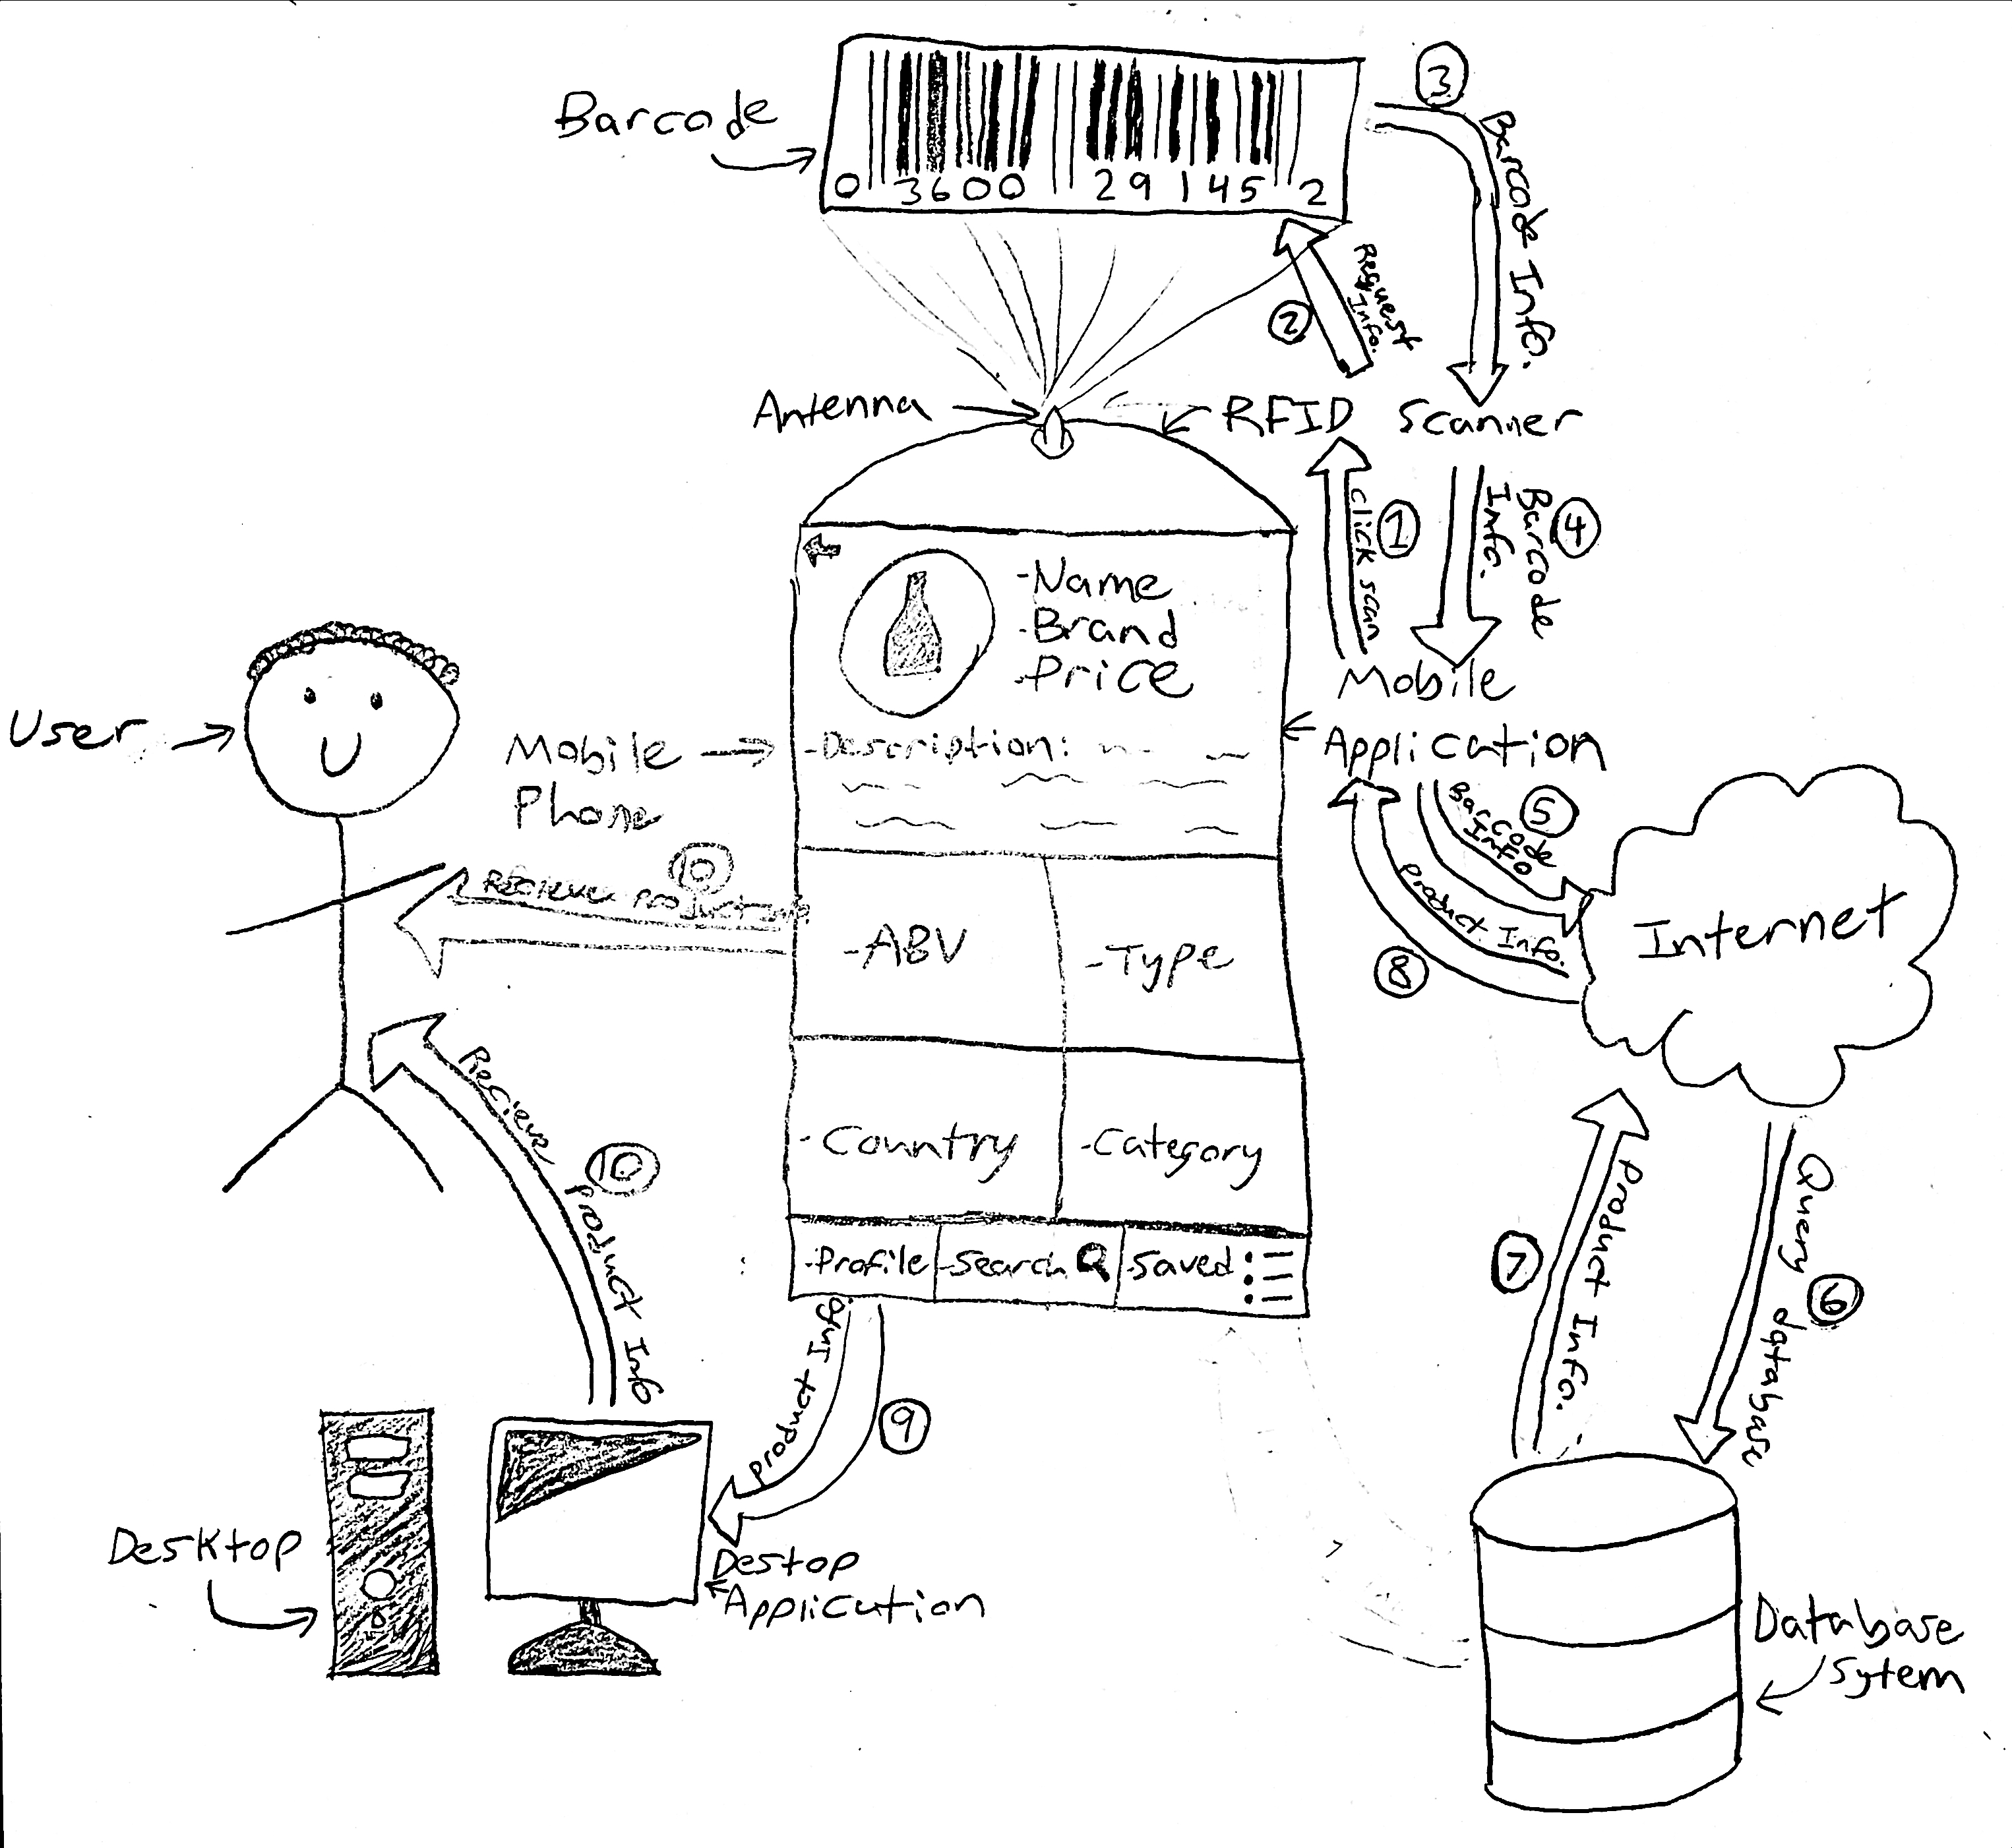
\includegraphics[width=0.60\textwidth]{images/information_flow.jpg}
   	\caption{Information Flow of Swift Scan}
\end{figure}
\vspace{0.5 in}

The main features of the product include:
\begin{itemize}
    \item scans the bar code of any alcoholic beverage
    \item provides information about the product scanned including the brand, alcohol type, category, price (depending on location), ABV, country, etc.
\end{itemize}

\subsection{External Inputs \& Outputs}
Here is a list of data/information flow components:
\begin{itemize}
    \item Barcode Info (Figure 2)
    \begin{itemize}
        \item Description: This information is collected from the barcode by the RFID reader and flows to the mobile phone and then to the database
        \item Use: This will be used to query the database for a product
    \end{itemize}
    \item Product Info (Figure 2)
    \begin{itemize}
        \item Description: This information will be sent from the database system to the mobile to device to be viewed by the user. The information is then synced with the desktop version of the software.
        \item Use: This allows the user to view the information corresponding to the scanned product on their mobile phone or desktop.
    \end{itemize}
\end{itemize}

\subsection{Product Interfaces}
The critical inputs and outputs are the screen to view product information and the camera/RFID reader will allow the user to collect the data. The user will have a simple and easy-to-use interface on their mobile device and desktop browser. The interface will include a profile page, scan page, product page, saved list page, settings, and much more (Figure 3). The administrators will run the database to keep products up-to-date and software like Android studio to make updates. The maintainers will resolve any bugs get reported on GitHub. Here is a mock-up of the mobile interface:
\begin{figure}[h!]
	\centering
   	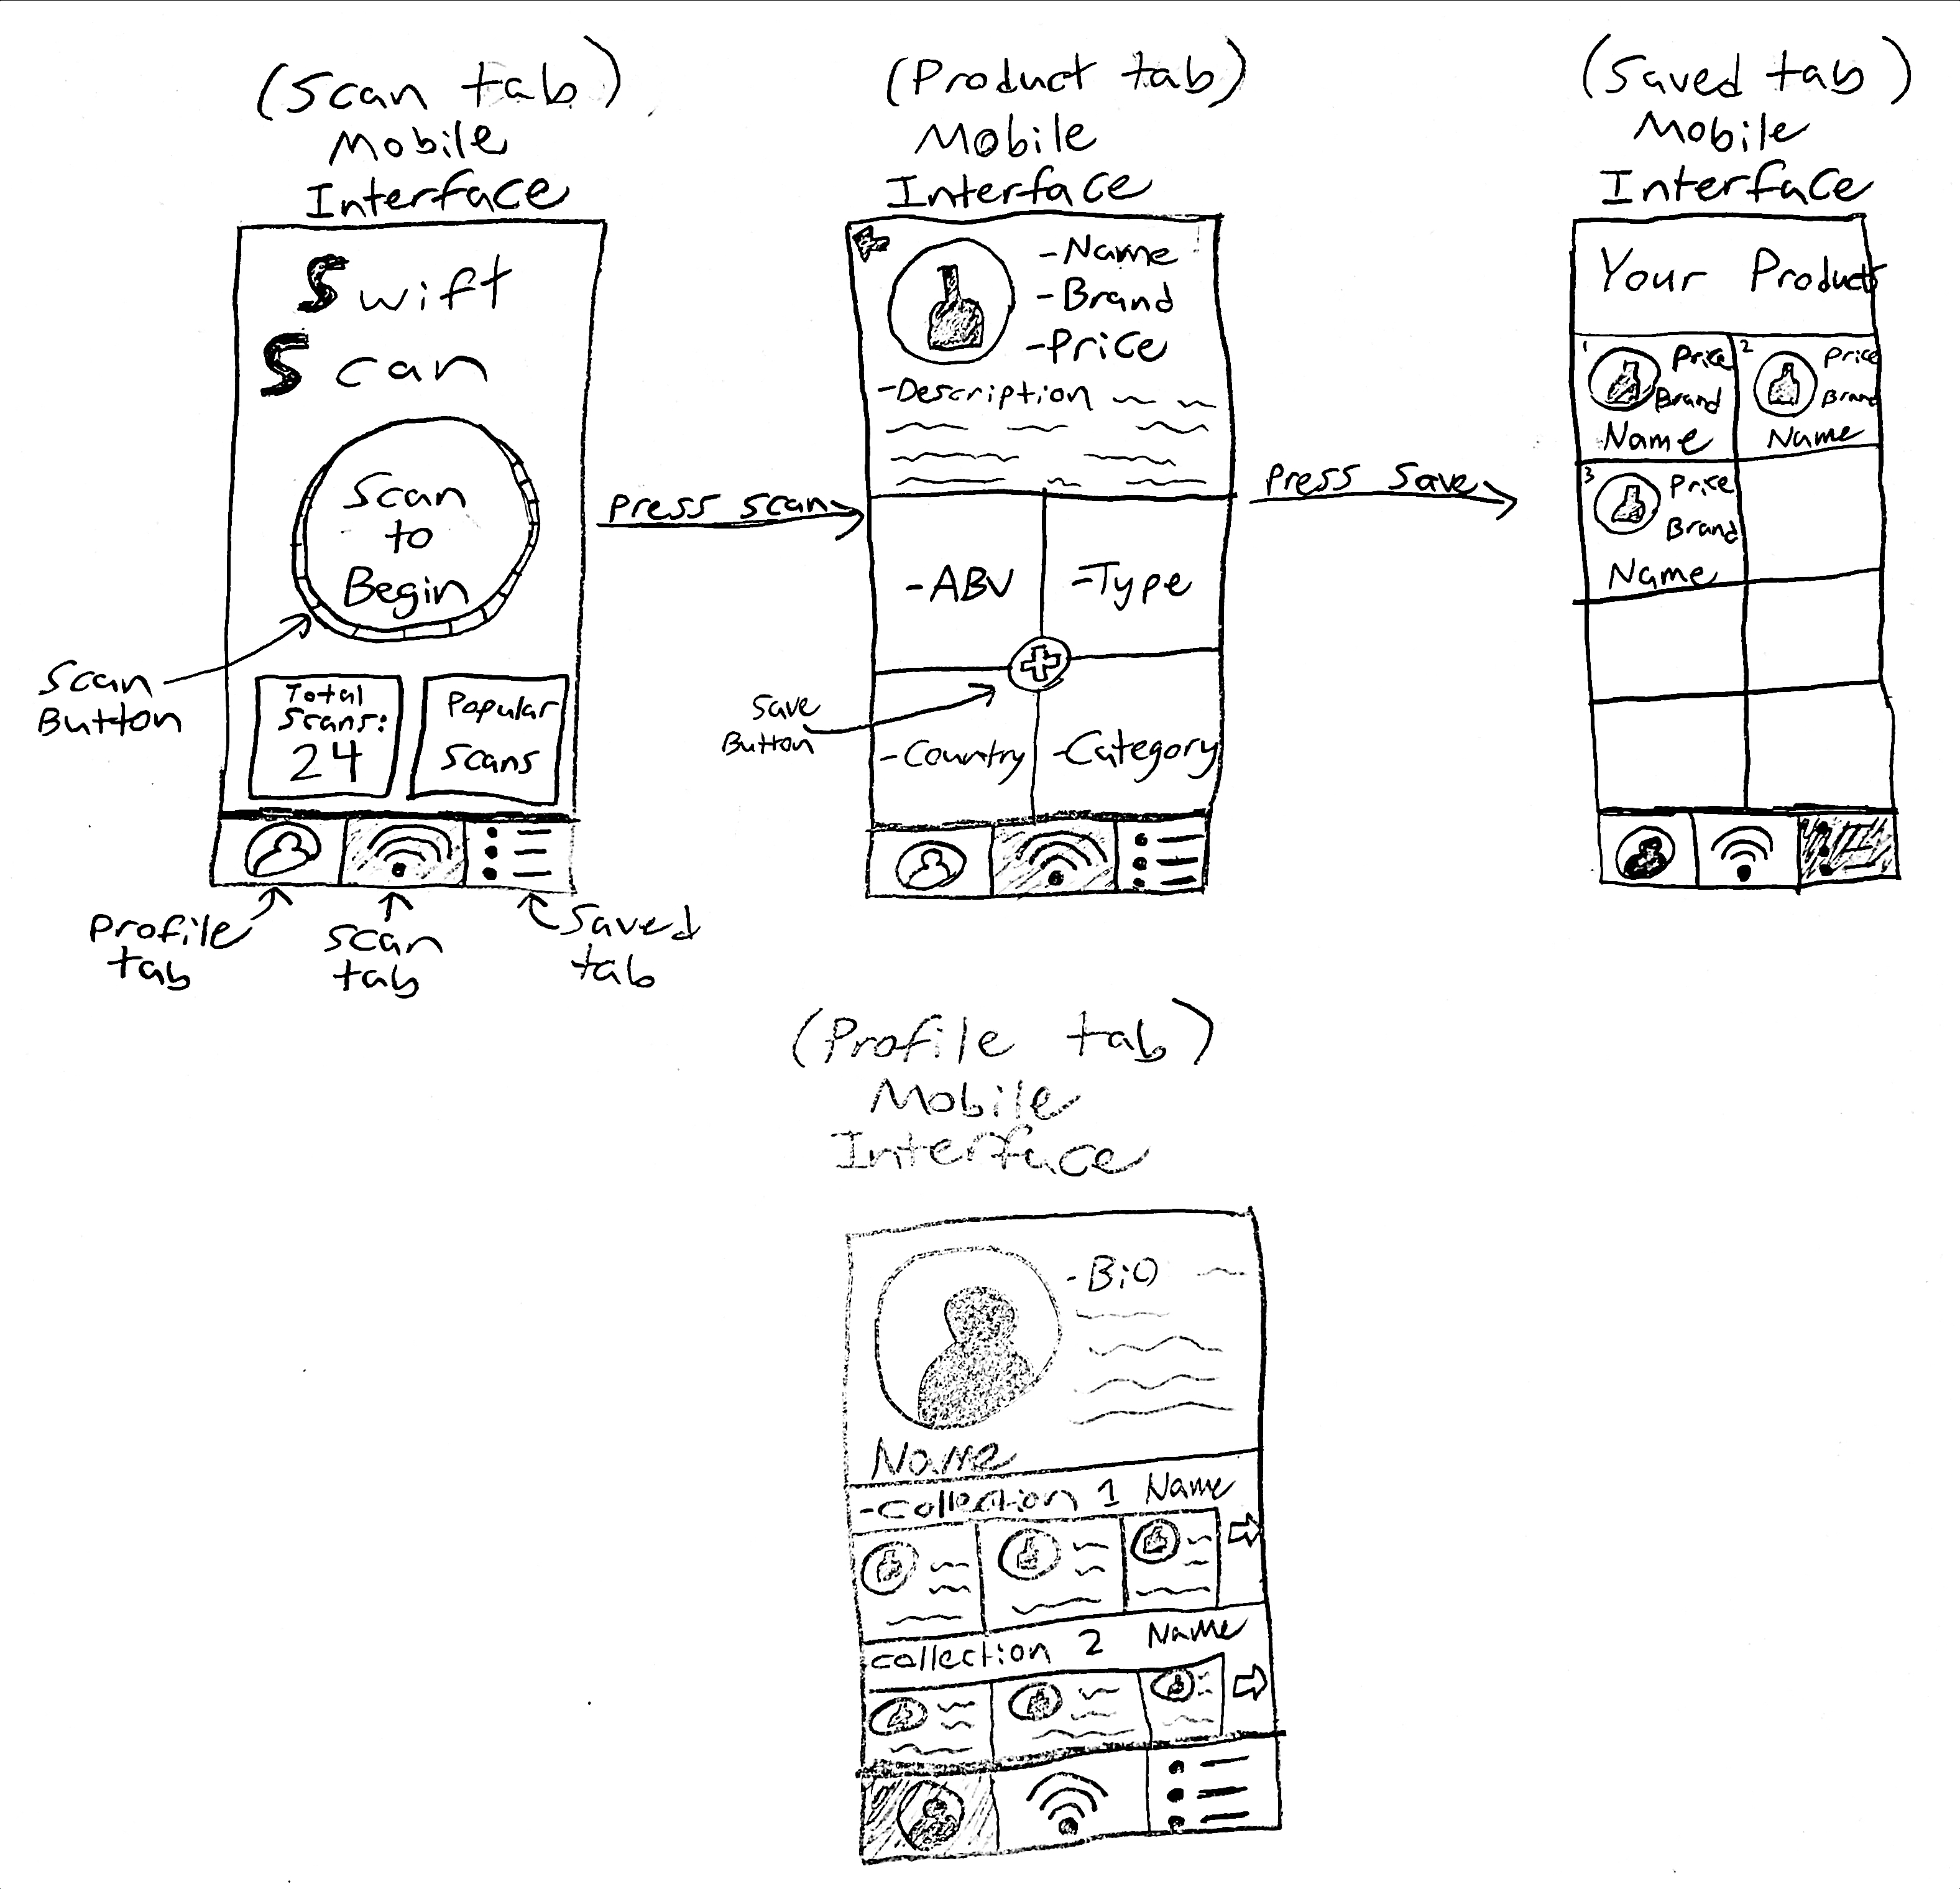
\includegraphics[width=0.60\textwidth]{images/mobile_interface.jpg}
   	\caption{Mobile Interface of Swift Scan}
\end{figure}

\newpage
\section{Customer Requirements}
Swift Scan will include a variety of user features including a mobile interface, desktop interface, and access to product information on a multitude of alcoholic beverages.

\subsection{Mobile Application}
\subsubsection{Description}
The mobile interface will be an application for Android. It will include features for scanning products, creating a profile page, settings page, product page, and saved products list. These features will allow users to scan products and then save their items into a personal collection. From their phone, using the camera or other scanner, they will be able to easily scan products. The GUI will have a red (\#D11313) and white (\#FFFFFF) color scheme.

\subsubsection{Source}
The source of this requirement comes from the specified team member (Jacob Wilkins).

\subsubsection{Constraints}
Some constraints include making sure the user is 21 or over, making sure the cost to produce is under the \$800 budget, making sure the customer information is safe and secure, and making sure the content on the application is appropriate.

\subsubsection{Standards}
To keep user information safe, we will apply signature-based permissions and use implicit intents. In addition, we will disallow access to the app's content provider.

\subsubsection{Priority}
Critical

\subsection{Web Application}
\subsubsection{Description}
The desktop interface will have the same features as the mobile interface except for the ability to scan. All scans from the mobile application will be synced with the desktop version so that the user can seamlessly go back and forth between apps. The GUI will have a red (\#D11313) and white (\#FFFFFF) color scheme.
\subsubsection{Source}
The source of this requirement comes from the specified team member (Jacob Wilkins).
\subsubsection{Constraints}
Some constraints include making sure the user is 21 or over, making sure the cost to produce is under the \$800 budget, making sure the customer information is safe and secure, and making sure the content on the application is appropriate.
\subsubsection{Standards}
The web application will use OWASP standards to make it secure for the user.
\subsubsection{Priority}
Moderate

\newpage
\section{Packaging Requirements}
The Beverage Invetory App (Swift Scan) will be available for download through GitHub for Android.  The GitHub link to download the Android app will be made available once the app has been fully tested and developed.  In addition, a desktop application will also be made available to download from GitHub and will need to be installed on a PC running Windows OS.  The desktop application will be an executable file so it can properly run on Windows OS.  The main purpose of the desktop application is for the user to have administrative privileges and access to adding, deleting, or modifying records from the central database that'll store all the information for any beverage.  Both the Android and desktop applications need to be both installed on an Android smartphone and Windows OS, respectively, in order for Swift Scan to function properly.  The RFID scanner device for the Android app will be packaged in a box with the name and logo of the application, Swift Scan.  An instruction manual will be included with the RFID scanner with information for both the Android and desktop applications.

\subsection{Requirement Name}
\subsubsection{Description}

\subsubsection{Source}
Customer, which will be Professor Chris Conly.
\subsubsection{Constraints}
For packaging requirements, the ideal constraint that we might run into is the shortage of barcode scanners in the market that could make it difficult to find and purchase a barcode scanner that is convenient for the customer.
\subsubsection{Standards}
Barcode scanner will meet the requirements to scan barcodes that are part of the EAN/UPC standard, which will scan 1D barcodes from the beverage products.
\subsubsection{Priority}
High

\newpage
\section{Performance Requirements}
Include a header paragraph specific to your product here. Performance requirements address items such as: how fast specific critical operations must complete; how long it takes to start/stop activities; how long the battery must last; maximum time it must take to set up; etc.

During the developmental stages of Swift Scan, the Android and Desktop apps will be tested for performance to make sure that information storage and retrieval are executed fast when the user interacts with the GUI.  The Android app, 

\subsection{Requirement Name}
\subsubsection{Description}
Detailed requirement description...
\subsubsection{Source}
Source
\subsubsection{Constraints}
Detailed description of applicable constraints...
\subsubsection{Standards}
List of applicable standards
\subsubsection{Priority}
Priority

\newpage
\section{Safety Requirements}
The project is based on software so there are not much potential safty requirements.But some of them may be  exposure to laser beam if used.
\subsection{Laboratory equipment lockout/tagout (LOTO) procedures}
The laboratory is located at Enginerring research building 203. The lab equipments used is a computer since it is a software project.
\subsubsection{Description}
 As our product is Beer Inventory app; It is mainly based on software rather than hardware. We are using Scanner, android app, cellphone. There is not much safety requirements, but just one no direct eye exposure to scanner/laser beams. 
\subsubsection{Source}
If we look for source, it might be Senior design laboratory policy or course instructor Chris Conly. 
\subsubsection{Constraints}
While Connecting Scanner with Desktop and other devices, and other equipment usages. Similarly, while testing Beer collection will be limited to availability of Course instructor.
\subsubsection{Standards}
Standards: NFPA 70E 2012; Arc flash code distributed by NFPA(national fire protection energy).
\subsubsection{Priority}
It is moderate.


\newpage
\section{Maintenance \& Support Requirements}
The database will required to have a monthly check in order to see if there is any type of fragmentation and the check the integrity of the whole database. MySQL comes with a Workspace that can be used to these routines or the command line interface can be used as well. A small guide will be given to demonstrate how to do these routines.

\subsection{Data Base Maintenance and Support}
\subsubsection{Description}
Databases such mysql require regular maintenance which has four main categories: Index Fragmentation, Log File Maintenance, File/Data Compaction and Integrity Check.

\textbf{1. Index Defragmentation:}
SQL databases contain objects called ‘indexes’ that work a lot like the Dewey Decimal system of a library. Each table inside of your database contains at least one indexed column that we use when we need to search for a specific value (such as an Employee or a Work Code). Indexes store a sorted and partitioned copy of that data in an ultra-fast section of memory, so when ask SQL server for some specific data (such as ‘All time cards for employee ‘Joe Demo’), the database first scans the indexes for ‘Joe Demo’ to get all the row numbers for Joe’s time cards, then retrieves just those records for the application. Without an index, the database would have to read each and every single record in the table (in its entirety) to find all the records. A well-designed (and well maintained) index can improve the performance of a query by 1,000 fold or more. So creating and maintaining indexes are extremely important.

One of the things that happens to indexes are that they get fragmented, just like your hard disk does. So rather than the index being in one continuous part of memory, it is divided into numerous different parts (sometimes THOUSANDS of parts) and stored wherever there is space. And just like when your computer’s hard disk is fragmented, your database becomes extremely lethargic. In order to fix this fragmentation, our maintenance plan evaluates each index for its size, use, and fragmentation level and will either perform a INDEX REORGANIZE, an INDEX REBUILD ONLINE, or even an INDEX REBUILD OFFLINE depending how bad the index is.

 

\textbf{2. Log File Maintenance:}
SQL Databases contain a ‘Log File’ that keeps track of every single transaction that happens in the database. Using these log files, you can actually restore a database to the state it was at any point in time before. So if something bad happens to your database (either corruption, accidentally, or maliciously), you can recover your data as it was the instant before the event happened. So the Log files are extremely important parts of the system, and they require their own special maintenance as well.

Log files automatically grow as you add more and more data to your database. Each time the file grows, it creates a ‘Virtual Log File’ (VLF) inside that it uses to store data. Using these VLFs the SQL Server is able to find a single operation in the log file much, much faster than if it had to scan the entire log file. The downside to this is that if there are too many VLFs, the time it takes to insert data into the log file can actually increase, which harms performance. Part of our maintenance routine is to scan these VLFs and see if they are hurting performance. If the maintenance routine determines that they are, then we adjust several factors of the log file, including how large each increment is when the log file grows. We can then compact these VLFs together to regain our lost performance (and without losing any log data).

 

\textbf{3. File/Data Compaction:}
As you use your SQL database, the file size both grows and shrinks. Each time the file needs more space, it grows by a certain increment. And as data is added to the database (as a chunk), it is saved into any spot that has enough memory to store that chunk. Unfortunately, the data is not always stored close to other data from the same table. The data itself becomes fragmented, just like the indexes we talked about before. In order to resolve this issue, we run what is called a ‘Data Compaction’, which reorganizes the file by grouping all associated data together. This not only groups data together, but it can also free up space inside the file as well, which can then be reclaimed by the operating system as free disk space on your hard disc.

 

\textbf{4. Integrity Check:}
Over time, your database will go through numerous changes. Data will be added and removed, tables will be added, modified, and removed. The database’s overall schema will change. Indexes will be added, rebuild, deleted, and re-created. Data columns will be added, modified, and removed. The database will go through thousands upon thousands of changes just as a natural course of its lifespan. But each change, no matter how small, has the potential to introduce corruption into the database. Indexes can have corrupt pages, table can have bad records, the schema can contain inaccurate references. These different types of corruption can cause anything from simple performance issues to complete schema failure and catastrophic data loss. But this is where the Integrity Check comes into play. The Database Integrity Check examines and analyzes the database in its entirety, and can detect and repair most any corruption it comes across. The database integrity check should be run on a regular, reoccurring, weekly schedule. The Integrity Check is your best weapon to prevent catastrophic data loss. Mysql workSpace has a built in Integrity Check that any OTP user with Admin rights can run on demand. If any corruption was detected or repaired, WorkSpace will immediately inform the user of the details, severity, and actions taken. In nearly all cases, that is where the corruption will end, and there will be no need for further action. But if you run an integrity check and WorkSpace reports that an issue was detected but was not resolved, please contact the Office Tools Technical Support team immediately. Our data specialists have decades of experience working with SQL Server databases and have been able to recover data that others though was completely irrecoverable.
\subsubsection{Source}
MySQL Reference Manual
\subsubsection{Constraints}
Database maintenance cannot be done remotely, an user with admin rights is needed to perform the maintenance.
\subsubsection{Standards}
None
\subsubsection{Priority}
High
\newpage
\section{Other Requirements}
The system will be able to run on Windows 10, Linux and Mac OS. The desktop application will be written using JAVA in a way that it can run on any platform running JAVA SE 12. 

\subsection{Porting Management Application to other Operative Systems}
\subsubsection{Description}
The desktop application will be made in JAVA SE 12 in a 64 bit machine. Any machine that can install the most recent version of JAVA and has a 64 bit architecture will run the desktop application. The source will be stored in a repository in GitHub and when the code is run, it will check to see if it is possible to run the app in the host machine.
\subsubsection{Source}
Source
\subsubsection{Constraints}
Java is installed in different places depending of the OS which can make it difficult for the program to work out of the box. There are new releases of Java released often so the source must be updated every time there is a new release.
\subsubsection{Standards}
Every source code file should begin with a file comment block describing the contents.
\subsubsection{Priority}
High
\newpage
\section{Future Items}
In this last section, you will reiterate all requirements that are listed as priority 5. This is repetitive, but necessary as a concise statement of features/functions that were considered/discussed and documented herein, but will NOT be addressed in the prototype version of the product due to constraints of budget, time, skills, technology, feasibility analysis, etc. Use the following format for this section.

\subsection{Requirement Name}

\subsubsection{Description}
Detailed requirement description...
\subsubsection{Source}
Source
Christopher Conly
\subsubsection{Constraints}

Detailed description of applicable constraints...
\subsubsection{Standards}
A precise brewing inventory app with various options.
List of applicable standards
\subsubsection{Priority}
Priority
Search types option available such as best by date, style, name.
Able to pull up information using barcode ot the name 

\newpage

%%% References
\bibliographystyle{plain}
\bibliographystyle{reference/IEEEtran_custom}
\bibliography{reference/refs}{}

\end{document}